\documentclass[10pt,a4paper]{article}
\usepackage[utf8]{inputenc}
\usepackage[spanish]{babel}
\usepackage{a4wide}
\usepackage[sinEntregas]{caratula}
\usepackage{ulem}
\usepackage{marginnote}
\usepackage{fancyhdr}
\usepackage{lastpage}
\usepackage{float}
\usepackage{tikz}

\pagestyle{fancy}
\thispagestyle{fancy}
\addtolength{\headheight}{1pt}
\lhead{Bases de Datos}
\rhead{TP2}
\cfoot{\thepage /\pageref{LastPage}}
\renewcommand{\thesubsubsection}{\thesubsection.\alph{subsubsection}}

\title{Bases de Datos - TP 2}
\author{Bases de Datos, DC, UBA.}

\begin{document}

\fecha{20 de junio de 2015}

\materia{Bases de Datos}
%\submateria{Trabajo Pr\'actico Nº1}
\titulo{Web Semántica}

\integrante{Allocati, Federico}{682/11}{fede.allocati@gmail.com}
\integrante{Izcovich, Sabrina}{550/11}{sizcovich@gmail.com}
\integrante{Pernigotti, Santiago}{870/11}{spernigotti@hotmail.com}
\integrante{Romano, Germán}{786/11}{romano.german@live.com.ar}

\maketitle

\tableofcontents

\newpage

\section{Introducción}

El trabajo práctico se basa en un análisis enfocado en el tema de \textit{Semántica Web}. Para la realización del mismo, basamos nuestra investigación en la tesis\footnote{http://dc.uba.ar/inv/tesis/licenciatura/2013/bursztyn.pdf} presentada por Damián A. Bursztyn en el año 2013 sobre Optimización de consultas RDF reformuladas.

En lo que sigue, explicaremos los conceptos de Semántica Web y sus problemáticas, como también de RDF, mecanismo que ayuda a convertir la Web en una infraestructura global en la que es posible compartir, y reutilizar datos y documentos entre diferentes tipos de usuarios.

\newpage
\section{Semántica Web}
La semántica web consiste en una Semántica Extendida dotada de mayor significado gracias a una información mejor definida. Su utilidad principal es encontrar soluciones a problemas habituales en la búsqueda de información gracias a la utilización de una infraestructura común mediante la cual se procesa y transfiere la información de una manera sencilla. Esta Web extendida y basada en el significado, se apoya en lenguajes universales que resuelven los problemas ocasionados por una Web carente de semántica en la que, en ocasiones, el acceso a la información se convierte en una tarea difícil y frustrante.

\subsection{Ejemplo}

\begin{figure}[H] %[h] Aqui [b] para button [t] para top
\begin{center}
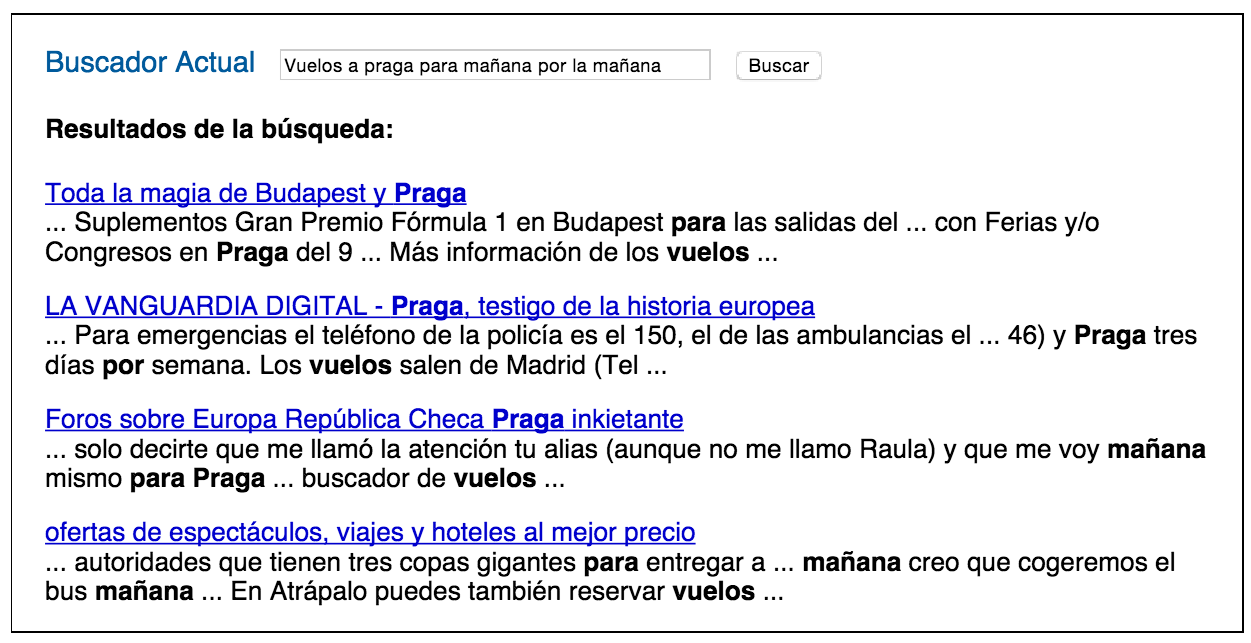
\includegraphics[width=400pt]{imgs/resultadoNormal}
\caption{Resultados obtenidos con un buscador normal.}
\end{center}
\end{figure}
\begin{figure}[H] %[h] Aqui [b] para button [t] para top
\begin{center}
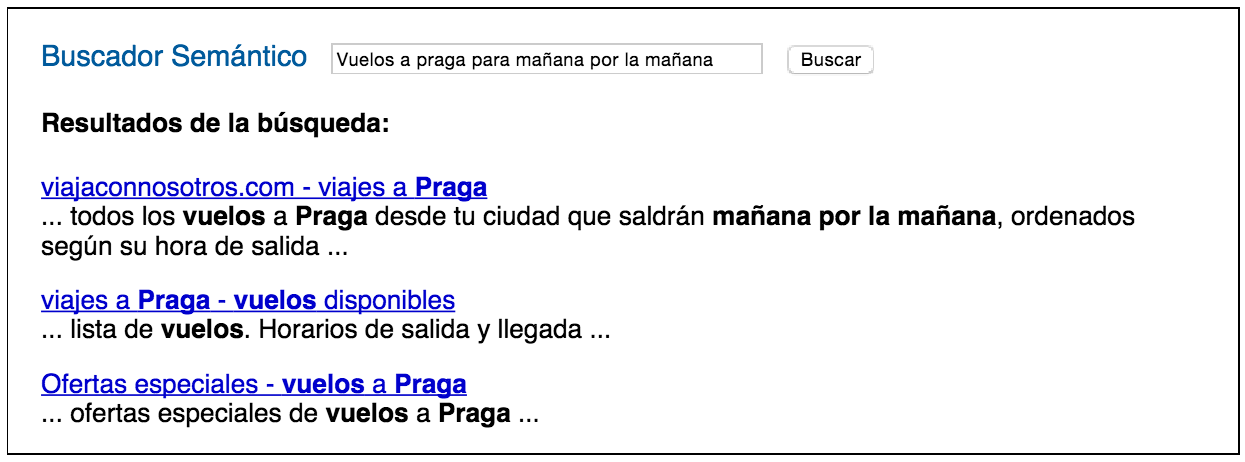
\includegraphics[width=400pt]{imgs/resultadoSemantico}
\caption{Resultados obtenidos con un buscador semántico.}
\end{center}
\end{figure}
\newpage
\section{Problemas de la Web Semántica}
En el último tiempo, el uso de Web Semántica creció enormemente e impulsó la necesidad de emplear técnicas eficientes y escalables para responder a las consultas RDF sobre una gran cantidad de datos heterogéneos. Una posible solución a este problema consiste en traducir las consultas RDF en consultas SQL para ejecutarlas en los sistemas de gestión de bases de datos relacionales (RDBMS). Sin embargo, las bases de datos para Web Semántica complican a las tecnologías clásicas de gestión de datos que no tienen en cuenta los datos implícitos durante la evaluación de consultas. Una solución a esto es reformular la consulta entrante para luego traducirla en una consulta SQL que, al ser evaluada por el RDBMS, devuelve las respuestas completas. El problema que esta solución presenta es de rendimiento debido a la longitud sintáctica de las consultas SQL que resultan de reformulación. Los RDBMSs no son capaces de optimizar eficientemente estas consultas, por lo que en algunos casos fallan o registran tiempos elevados de evaluación.

\newpage
\section{RDF}
Un set de datos RDF consiste en datos explícitos e implícitos presentes en la base de datos, dados por restricciones semánticas que deben cumplir. Dichos datos son obtenidos por un proceso que considera las restricciones para inferir todas las posibles consecuencias de la base de datos existente.

\newpage
\section{Mecanismos de conversión de la Web}
Para obtener una adecuada definición de los datos, la Web Semántica utiliza esencialmente RDF, SPARQL, y OWL, mecanismos que ayudan a convertir la Web en una infraestructura global en la que es posible compartir, y reutilizar datos y documentos entre diferentes tipos de usuarios.

\begin{itemize}
\item \textbf{RDF} proporciona información descriptiva simple sobre los recursos que se encuentran en la Web y que se utiliza, por ejemplo, en catálogos de libros, directorios, colecciones personales de música, fotos, eventos, etc.
\item \textbf{SPARQL} es lenguaje de consulta sobre RDF, que permite hacer búsquedas sobre los recursos de la Web Semántica utilizando distintas fuentes datos.
\item \textbf{OWL} es un mecanismo para desarrollar temas o vocabularios específicos en los que asociar esos recursos. Lo que hace OWL es proporcionar un lenguaje para definir ontologías estructuradas que pueden ser utilizadas a través de diferentes sistemas. Las ontologías, que se encargan de definir los términos utilizados para describir y representar un área de conocimiento, son utilizadas por los usuarios, las bases de datos y las aplicaciones que necesitan compartir información específica, es decir, en un campo determinado como puede ser el de las finanzas, medicina, deporte, etc. Las ontologías incluyen definiciones de conceptos básicos en un campo determinado y la relación entre ellos.
\end{itemize}

\newpage

\section{Referencias}

\begin{itemize}
\item The World Wide Web Consortium (W3C). http://www.w3c.es/Divulgacion/GuiasBreves/WebSemantica
\item http://jplu.developpez.com/tutoriels/web-semantique/introduction/
\end{itemize}

\end{document}